\documentclass{article}
\usepackage{graphicx}
\usepackage{subcaption}
\usepackage[margin=1in]{geometry}

\begin{document}

\begin{figure}[ht]

\begin{subfigure}{.83\linewidth}
	\centering
	\begin{subfigure}{0.4\linewidth}
		\centering
		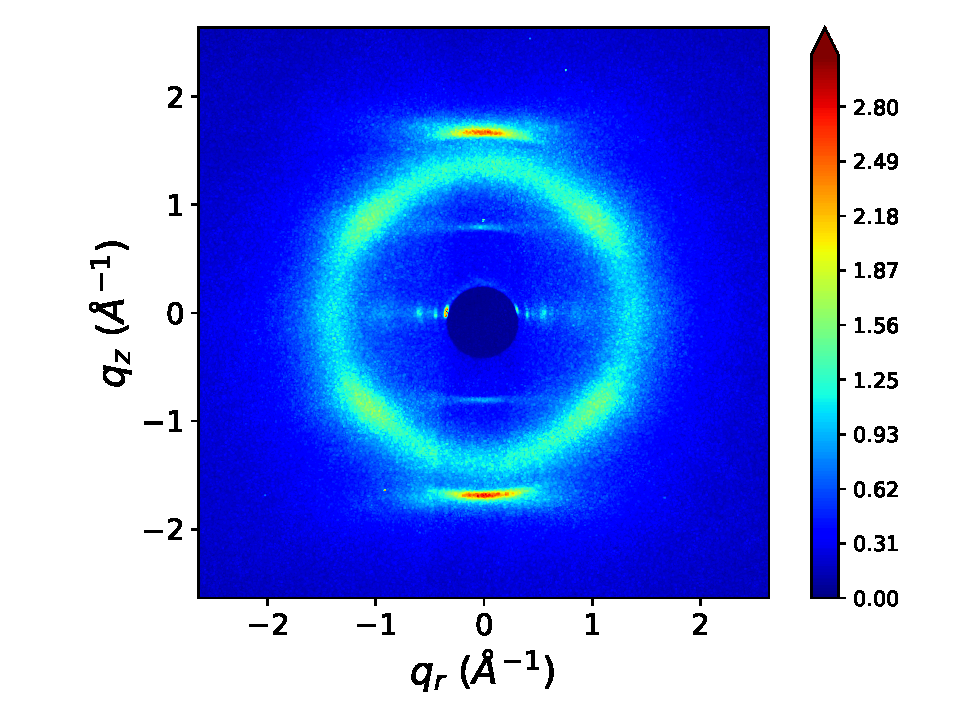
\includegraphics[width=\linewidth, trim={2.5cm 0 4cm 2cm}, clip]{WAXS_raw.png}%
		\caption{}~\label{fig:raw_waxs}	
	\end{subfigure}%
	\begin{subfigure}{0.4\linewidth}
		\centering
		\includegraphics[width=\linewidth, trim={2cm 0 2.5cm 1.25cm}, clip]{rzplot_offset.png}
		\caption{}~\label{fig:rz_offset}
	\end{subfigure}
	\begin{subfigure}{0.4\linewidth}
		\centering
		\includegraphics[width=\linewidth, trim={2cm 0 2.5cm 1.25cm}, clip]{rzplot_layered.png}
		\caption{}~\label{fig:rz_layered}
	\end{subfigure}%
	\begin{subfigure}{0.4\linewidth}
		\centering
		\includegraphics[width=\linewidth, trim={2cm 0 2.5cm 1.25cm}, clip]{rzplot_disordered.png}
		\caption{}~\label{fig:rz_disordered}
	\end{subfigure}
\end{subfigure}%
\begin{subfigure}{0.14\linewidth}
	\centering
	\vspace{-1cm}
	\includegraphics[width=\linewidth]{colorbar_jet.png}
\end{subfigure}
\caption{(a) Experimental 2D WAXS data contains 5 major reflections which we aim to match. The remaining 
three images are diffraction patterns simulated from MD trajectories. (b) The parallel displaced
configuration gives rise to all reflections of interest. (c) The sandwiched configurations gives rise to a
pattern with all major reflections except R-helix. R-spots is strong relative to R-alkanes in comparison
to the parallel displaced configuration. (d) The disordered pore configuration creates a pattern with only
R-alkanes and R-pores in common with experiment}~\label{fig:xrd}
\end{figure}

\end{document}
